\makeatletter
\@ifundefined{standalonetrue}{\newif\ifstandalone}{}
\@ifundefined{section}{\standalonetrue}{\standalonefalse}
\makeatother
\ifstandalone
\documentclass[11pt]{report}
\usepackage{textcase}
%\usepackage{hyperref}
%\hypersetup{breaklinks=true}


% Added packages
\usepackage[usenames]{color}
\usepackage{amsfonts, amsmath, amssymb, graphics}

% NOTE: bibentry MUST appear before the hyperref or build will fail
\usepackage{bibentry}
\nobibliography*
\usepackage[square,sort,comma,numbers]{natbib}
  
\usepackage{float}
\usepackage[
	hidelinks,%
    %hyperindex=true,		% Make numbers of index links as well
   	backref=page, 		% Provide page listing where refs occur in the bibliography
	%breaklinks=true,
    %colorlinks,%
    %citecolor=green,%
    %filecolor=blue,%
    %linkcolor=red,%
    %urlcolor=red, 
]{hyperref}

\usepackage{dsfont}
%%%% USEPACKAGES for MACROS %%%%%
\usepackage{algpseudocode}
\usepackage[chapter]{algorithm}
%\usepackage{caption}
\usepackage{subcaption}
\usepackage{url}

\usepackage{array}
\usepackage{arydshln}
\usepackage{multirow}
\usepackage{multicol}
%\usepackage[section]{placeins}

\usepackage[usenames,dvipsnames]{color}
%\usepackage[english]{babel}
\usepackage{tabularx}
\usepackage{soul}
\usepackage{xparse}
\usepackage{listings}
%\usepackage[normalem]{ulem}



%%%%%%%%%%%%%%%
% Show a list of items "todo" or "done" 
% USAGE: 
% \begin{todolist} 
% 	\todo Something not finished
% 	\done Something finished
% \end{todolist} 
\newenvironment{todolist}{%
  \begin{list}{}{}% whatever you want the list to be
  \let\olditem\item
  \renewcommand\item{\olditem \textcolor{red}{(TODO)}: }
  \newcommand\todo{\olditem \textcolor{red}{(TODO)}: }
   \newcommand\done{\olditem \textcolor{ForestGreen}{(DONE)}: }
}{%
  \end{list}
} 
%%%%%%%%%%%%%%%

%%%%%%%%%%%%%%%
% Show a Author's Note
% USAGE: 
% \incomplete[Optional footnote message to further clarify note]{The text which is currently not finished}
\DeclareDocumentCommand \incomplete{ o m }
{%
\IfNoValueTF {#1}
{\textcolor{red}{Incomplete: \ul{#2}}} 
{\textcolor{red}{Incomplete: \ul{#2}}\footnote{Comment: #1}}%
}
%%%%%%%%%%%%%%%



%%%%%%%%%%%%%%%
% Show a Author's Note
% USAGE: 
% \authnote[Optional footnote message to further clarify note]{The note to your readers}
\DeclareDocumentCommand \authnote { o m }
{%
\IfNoValueTF {#1}
{\textcolor{blue}{Author's Note: \ul{#2}}} 
{\textcolor{blue}{Author's Note: \ul{#2}}\footnote{Comment: #1}}%
}
%%%%%%%%%%%%%%%



%%%%%%%%%%%%%%%
% Strike out text that doesn't belong in the paper
% USAGE: 
% \strike[Optional footnote to state why it doesn't belong]{Text to strike out}
\DeclareDocumentCommand \strike { o m }
{%
\setstcolor{Red}
\IfNoValueTF {#1}
{\textcolor{Gray}{\st{#2}}} 
{\textcolor{Gray}{\st{#2}}\footnote{Comment: #1}}%
}
%%%%%%%%%%%%%%%

\definecolor{light-gray}{gray}{0.95}

\newcommand{\cbox}[3]{
\ \\
\fcolorbox{#1}{#2}{
\parbox{\textwidth}{
#3
}
}
}

% Setup an environment similar to verbatim but which will highlight any bash commands we have
\lstnewenvironment{unixcmds}[0]
{
%\lstset{language=bash,frame=shadowbox,rulesepcolor=\color{blue}}
\lstset{ %
language=sh,		% Language
basicstyle=\ttfamily,
backgroundcolor=\color{light-gray}, 
rulecolor=\color{blue},
%frame=tb, 
columns=fullflexible,
%framexrightmargin=-.2\textwidth,
linewidth=0.8\textwidth,
breaklines=true,
%prebreak=/, 
  prebreak = \raisebox{0ex}[0ex][0ex]{\ensuremath{\hookleftarrow}},
%basicstyle=\footnotesize,       % the size of the fonts that are used for the code
%numbers=left,                   % where to put the line-numbers
%numberstyle=\footnotesize,      % the size of the fonts that are used for the line-numbers
%stepnumber=2,                   % the step between two line-numbers. If it's 1 each line 
                                % will be numbered
%numbersep=5pt,                  % how far the line-numbers are from the code
showspaces=false,               % show spaces adding particular underscores
showstringspaces=false,         % underline spaces within strings
showtabs=false,                 % show tabs within strings adding particular underscores
frame=single,	                % adds a frame around the code
tabsize=2,	                % sets default tabsize to 2 spaces
captionpos=b,                   % sets the caption-position to bottom
breakatwhitespace=false,        % sets if automatic breaks should only happen at whitespace
}
} { }

% Setup an environment similar to verbatim but which will highlight any bash commands we have
\lstnewenvironment{cppcode}[1]
{
%\lstset{language=bash,frame=shadowbox,rulesepcolor=\color{blue}}
\lstset{ %
	backgroundcolor=\color{light-gray}, 
	rulecolor=\color[rgb]{0.133,0.545,0.133},
	tabsize=4,
	language=[GNU]C++,
%	basicstyle=\ttfamily,
        basicstyle=\scriptsize,
        upquote=true,
        aboveskip={1.5\baselineskip},
        columns=fullflexible,
        %framexrightmargin=-.1\textwidth,
       %framexleftmargin=6mm,
        showstringspaces=false,
        extendedchars=true,
        breaklines=true,
        prebreak = \raisebox{0ex}[0ex][0ex]{\ensuremath{\hookleftarrow}},
        frame=single,
        showtabs=false,
        showspaces=false,
        showstringspaces=false,
        numbers=left,                   % where to put the line-numbers
	numberstyle=\footnotesize,      % the size of the fonts that are used for the line-numbers
	stepnumber=4,                   % the step between two line-numbers. If it's 1 each line 
                                % will be numbered
	firstnumber=#1,
         numbersep=5pt,                  % how far the line-numbers are from the code
        identifierstyle=\ttfamily,
        keywordstyle=\color[rgb]{0,0,1},
        commentstyle=\color[rgb]{0.133,0.545,0.133},
        stringstyle=\color[rgb]{0.627,0.126,0.941},
}
} { }

% Setup an environment similar to verbatim but which will highlight any bash commands we have
\lstnewenvironment{mcode}[1]
{
\lstset{ %
	backgroundcolor=\color{light-gray}, 
	rulecolor=\color[rgb]{0.133,0.545,0.133},
	tabsize=4,
	language=Matlab,
%	basicstyle=\ttfamily,
        basicstyle=\scriptsize,
        upquote=true,
        aboveskip={1.5\baselineskip},
        columns=fullflexible,
        %framexrightmargin=-.1\textwidth,
       %framexleftmargin=6mm,
        showstringspaces=false,
        extendedchars=true,
        breaklines=true,
        prebreak = \raisebox{0ex}[0ex][0ex]{\ensuremath{\hookleftarrow}},
        frame=single,
        showtabs=false,
        showspaces=false,
        showstringspaces=false,
        numbers=left,                   % where to put the line-numbers
	numberstyle=\footnotesize,      % the size of the fonts that are used for the line-numbers
	stepnumber=4,                   % the step between two line-numbers. If it's 1 each line 
                                % will be numbered
	firstnumber=#1,
         numbersep=5pt,                  % how far the line-numbers are from the code
        identifierstyle=\ttfamily,
        keywordstyle=\color[rgb]{0,0,1},
        commentstyle=\color[rgb]{0.133,0.545,0.133},
        stringstyle=\color[rgb]{0.627,0.126,0.941},
}
} { }

\newcommand{\inputmcode}[1]{%
\lstset{ %
	backgroundcolor=\color{light-gray},  %
	rulecolor=\color[rgb]{0.133,0.545,0.133}, %
	tabsize=4, %
	language=Matlab, %
%	basicstyle=\ttfamily,
        basicstyle=\scriptsize, %
        %        upquote=true,
        aboveskip={1.5\baselineskip}, %
        columns=fullflexible, %
        %framexrightmargin=-.1\textwidth,
       %framexleftmargin=6mm,
        showstringspaces=false, %
        extendedchars=true, %
        breaklines=true, %
        prebreak = \raisebox{0ex}[0ex][0ex]{\ensuremath{\hookleftarrow}}, %
        frame=single, %
        showtabs=false, %
        showspaces=false, %
        showstringspaces=false,%
        numbers=left,                   % where to put the line-numbers
	numberstyle=\footnotesize,      % the size of the fonts that are used for the line-numbers
	stepnumber=4,                   % the step between two line-numbers. If it's 1 each line 
                                % will be numbered
         numbersep=5pt,                  % how far the line-numbers are from the code
        identifierstyle=\ttfamily, %
        keywordstyle=\color[rgb]{0,0,1}, %
        commentstyle=\color[rgb]{0.133,0.545,0.133}, %
        stringstyle=\color[rgb]{0.627,0.126,0.941} %
}
\lstinputlisting{#1}%
}

%\lstset{ %
%	backgroundcolor=\color{light-gray}, 
%	rulecolor=\color[rgb]{0.133,0.545,0.133},
%	tabsize=4,
%	language=Matlab,
%%	basicstyle=\ttfamily,
%        basicstyle=\scriptsize,
%        upquote=true,
%        aboveskip={1.5\baselineskip},
%        columns=fullflexible,
%        %framexrightmargin=-.1\textwidth,
%       %framexleftmargin=6mm,
%        showstringspaces=false,
%        extendedchars=true,
%        breaklines=true,
%        prebreak = \raisebox{0ex}[0ex][0ex]{\ensuremath{\hookleftarrow}},
%        frame=single,
%        showtabs=false,
%        showspaces=false,
%        showstringspaces=false,
%        numbers=left,                   % where to put the line-numbers
%	numberstyle=\footnotesize,      % the size of the fonts that are used for the line-numbers
%	stepnumber=4,                   % the step between two line-numbers. If it's 1 each line 
%                                % will be numbered
%	firstnumber=#1,
%         numbersep=5pt,                  % how far the line-numbers are from the code
%        identifierstyle=\ttfamily,
%        keywordstyle=\color[rgb]{0,0,1},
%        commentstyle=\color[rgb]{0.133,0.545,0.133},
%        stringstyle=\color[rgb]{0.627,0.126,0.941},
%}


\newcommand{\Laplacian}[1]{\nabla^2 #1}

% set of all nodes received and contained on GPU
\newcommand{\setAllNodes}[0]{\mathcal{G}}
% set of stencil centers on GPU
\newcommand{\setCenters}[0]{\mathcal{Q}}
% set of stencil centers with nodes in \setDepend
\newcommand{\setBoundary}[0]{\mathcal{B}}
% set of nodes received by other GPUs
\newcommand{\setDepend}[0]{\mathcal{R}}
% set of nodes sent to other GPUs
\newcommand{\setProvide}[0]{\mathcal{O}}


\newcommand{\toprule}[0]{\hline}
\newcommand{\midrule}[0]{\hline\hline}
\newcommand{\bottomrule}[0]{\hline}

\newcolumntype{C}{>{\centering\arraybackslash}b{1in}}
\newcolumntype{L}{>{\flushleft\arraybackslash}b{1.5in}}
\newcolumntype{R}{>{\flushright\arraybackslash}b{1.5in}}
\newcolumntype{D}{>{\flushright\arraybackslash}b{2.0in}}
\newcolumntype{E}{>{\flushright\arraybackslash}b{1.0in}}

\DeclareSymbolFont{AMSb}{U}{msb}{m}{n}
\DeclareMathSymbol{\N}{\mathbin}{AMSb}{"4E}
\DeclareMathSymbol{\Z}{\mathbin}{AMSb}{"5A}
\DeclareMathSymbol{\R}{\mathbin}{AMSb}{"52}
\DeclareMathSymbol{\Q}{\mathbin}{AMSb}{"51}
\DeclareMathSymbol{\PP}{\mathbin}{AMSb}{"50}
\DeclareMathSymbol{\I}{\mathbin}{AMSb}{"49}
%\DeclareMathSymbol{\C}{\mathbin}{AMSb}{"43}

%%%%%% VECTOR NORM: %%%%%%%
\newcommand{\vectornorm}[1]{\left|\left|#1\right|\right|}
\newcommand{\vnorm}[1]{\left|\left|#1\right|\right|}
\newcommand{\by}[0]{\times}
\newcommand{\vect}[1]{\mathbf{#1}}
%\newcommand{\mat}[1]{\mathbf{#1}} 

%\renewcommand{\vec}[1]{ \textbf{#1} }
%%%%%%%%%%%%%%%%%%%%%%

%%%%%%% THM, COR, DEF %%%%%%%
%\newtheorem{theorem}{Theorem}[section]
%\newtheorem{lemma}[theorem]{Lemma}
%\newtheorem{proposition}[theorem]{Proposition}
%\newtheorem{corollary}[theorem]{Corollary}
%\newenvironment{proof}[1][Proof]{\begin{trivlist}
%\item[\hskip \labelsep {\bfseries #1}]}{\end{trivlist}}
%\newenvironment{definition}[1][Definition]{\begin{trivlist}
%\item[\hskip \labelsep {\bfseries #1}]}{\end{trivlist}}
%\newenvironment{example}[1][Example]{\begin{trivlist}
%\item[\hskip \labelsep {\bfseries #1}]}{\end{trivlist}}
%\newenvironment{remark}[1][Remark]{\begin{trivlist}
%\item[\hskip \labelsep {\bfseries #1}]}{\end{trivlist}}
%\newcommand{\qed}{\nobreak \ifvmode \relax \else
%      \ifdim\lastskip<1.5em \hskip-\lastskip
%      \hskip1.5em plus0em minus0.5em \fi \nobreak
%      \vrule height0.75em width0.5em depth0.25em\fi}
%%%%%%%%%%%%%%%%%%%%%%

%
%\usepackage[algochapter]{algorithm2e}
%\usepackage[usenames]{color}
% colors to show the corrections
\newcommand{\red}[1]{\textbf{\textcolor{red}{#1}}}
\newcommand{\blue}[1]{\textbf{\textcolor{blue}{#1}}}
\newcommand{\cyan}[1]{\textbf{\textcolor{cyan}{#1}}}
\newcommand{\green}[1]{\textbf{\textcolor{green}{#1}}}
\newcommand{\magenta}[1]{\textbf{\textcolor{magenta}{#1}}}
\newcommand{\orange}[1]{\textbf{\textcolor{orange}{#1}}}
%%%%%%%%%% DK DK
% comments between authors
\newcommand{\toall}[1]{\textbf{\green{@@@ All: #1 @@@}}}
\newcommand{\toevan}[1]{\textbf{\red{*** Evan: #1 ***}}}
%\newcommand{\toevan}[1]{}  % USE FOR FINAL VERSION
\newcommand{\toe}[1]{\textbf{\red{*** Evan: #1 ***}}}
\newcommand{\tog}[1]{\textbf{\blue{*** Gordon: #1 ***}}}
%\newcommand{\togordon}[1]{\textbf{\blue{*** Gordon: #1 ***}}}
\renewcommand{\ge}[3]{{\textcolor{blue}{*** \textbf{Gordon:}\strike{#1} #2 ***}}\red{(#3)}}
\renewcommand{\ge}[3]{{\textcolor{blue}{#2}}}
\renewcommand{\ge}[3]{{\textcolor{Red}{#2}}}
\newcommand{\eb}[3]{{\textcolor{Red}{*** \textbf{Evan:}\strike{#1} #2 ***}}\red{(#3)}}
\renewcommand{\eb}[3]{{{\textcolor{Red}{#2}}}}
%\def\ge#1#2#3{}{\textbf{\blue{*** Gordon: #2 ***}}}{(#3)}
\newcommand{\gee}[1]{{\bf{\blue{{\em #1}}}}}
\newcommand{\old}[1]{}
\newcommand{\del}[1]{***#1*** }



% \DeclareMathOperator{\Sample}{Sample}
%\let\vaccent=\v % rename builtin command \v{} to \vaccent{}
%\renewcommand{\vec}[1]{\ensuremath{\mathbf{#1}}} % for vectors
\newcommand{\gv}[1]{\ensuremath{\mbox{\boldmath$ #1 $}}} 
% for vectors of Greek letters
\newcommand{\uv}[1]{\ensuremath{\mathbf{\hat{#1}}}} % for unit vector
\newcommand{\abs}[1]{\left| #1 \right|} % for absolute value
\newcommand{\avg}[1]{\left< #1 \right>} % for average
\let\underdot=\d % rename builtin command \d{} to \underdot{}
\renewcommand{\d}[2]{\frac{d #1}{d #2}} % for derivatives
\newcommand{\dd}[2]{\frac{d^2 #1}{d #2^2}} % for double derivatives
\newcommand{\pd}[2]{\frac{\partial #1}{\partial #2}} 
% for partial derivatives
\newcommand{\pdd}[2]{\frac{\partial^2 #1}{\partial #2^2}} 
\newcommand{\pdda}[3]{\frac{\partial^2 #1}{\partial #2 \partial #3}} 
% for double partial derivatives
\newcommand{\pdc}[3]{\left( \frac{\partial #1}{\partial #2}
 \right)_{#3}} % for thermodynamic partial derivatives
\newcommand{\ket}[1]{\left| #1 \right>} % for Dirac bras
\newcommand{\bra}[1]{\left< #1 \right|} % for Dirac kets
\newcommand{\braket}[2]{\left< #1 \vphantom{#2} \right|
 \left. #2 \vphantom{#1} \right>} % for Dirac brackets
\newcommand{\matrixel}[3]{\left< #1 \vphantom{#2#3} \right|
 #2 \left| #3 \vphantom{#1#2} \right>} % for Dirac matrix elements
\newcommand{\grad}[1]{\gv{\nabla} #1} % for gradient
\let\divsymb=\div % rename builtin command \div to \divsymb
\renewcommand{\div}[1]{\gv{\nabla} \cdot #1} % for divergence
\newcommand{\curl}[1]{\gv{\nabla} \times #1} % for curl
\let\baraccent=\= % rename builtin command \= to \baraccent
\renewcommand{\=}[1]{\stackrel{#1}{=}} % for putting numbers above =
\newcommand{\diffop}[1]{\mathcal{L}#1}
\newcommand{\boundop}[1]{\mathcal{B}#1}
\newcommand{\rvec}[0]{{\bf r}}

\newcommand{\Interior}[0]{\Omega}
\newcommand{\domain}[0]{\Omega}
%\newcommand{\Boundary}[0]{\partial \Omega}
\newcommand{\Boundary}[0]{\Gamma}

\newcommand{\on}[1]{\hskip1.5em \textrm{ on } #1}

\newcommand{\gemm}{\texttt{GEMM}}
\newcommand{\trmm}{\texttt{TRMM}}
\newcommand{\gesvd}{\texttt{GESVD}}
\newcommand{\geqrf}{\texttt{GEQRF}}


\newcommand{\minitab}[2][l]{\begin{tabular}{#1}#2\end{tabular}}
\newcommand{\comm}[1]{\textcolor{red}{\textit{#1}}}

\newcommand{\nfrac}[2]{
\nicefrac{#1}{#2}
%\frac{#1}{#2}
}

\usepackage{xparse}
\usepackage{soul}


%%%%%%%%%%%%%%%
% Show a Author's Note
% USAGE: 
% \incomplete[Optional footnote message to further clarify note]{The text which is currently not finished}
\DeclareDocumentCommand \incomplete{ o m }
{%
\IfNoValueTF {#1}
{\textcolor{red}{Incomplete: \ul{#2}}} 
{\textcolor{red}{Incomplete: \ul{#2}}\footnote{Comment: #1}}%
}
%%%%%%%%%%%%%%%



%%%%%%%%%%%%%%%
% Show a Author's Note
% USAGE: 
% \authnote[Optional footnote message to further clarify note]{The note to your readers}
\DeclareDocumentCommand \authnote { o m }
{%
\IfNoValueTF {#1}
{\textcolor{blue}{Author's Note: \ul{#2}}} 
{\textcolor{blue}{Author's Note: \ul{#2}}\footnote{Comment: #1}}%
}
%%%%%%%%%%%%%%%



%%%%%%%%%%%%%%%
% Strike out text that doesn't belong in the paper
% USAGE: 
% \strike[Optional footnote to state why it doesn't belong]{Text to strike out}
\DeclareDocumentCommand \strike { o m }
{%
\setstcolor{red}
\IfNoValueTF {#1}
{\textcolor{Gray}{\st{#2}}} 
{\textcolor{Gray}{\st{#2}}\footnote{Comment: #1}}%
}
%%%%%%%%%%%%%%%



%
% colors to show the corrections
\newcommand{\red}[1]{\textbf{\textcolor{red}{#1}}}
\newcommand{\blue}[1]{\textbf{\textcolor{blue}{#1}}}
\newcommand{\cyan}[1]{\textbf{\textcolor{cyan}{#1}}}
\newcommand{\green}[1]{\textbf{\textcolor{green}{#1}}}
\newcommand{\magenta}[1]{\textbf{\textcolor{magenta}{#1}}}
\newcommand{\orange}[1]{\textbf{\textcolor{orange}{#1}}}
%%%%%%%%%% DK DK
% comments between authors
\newcommand{\toall}[1]{\textbf{\green{@@@ All: #1 @@@}}}
\newcommand{\toevan}[1]{\textbf{\red{*** Evan: #1 ***}}}
%\newcommand{\toevan}[1]{}  % USE FOR FINAL VERSION
\newcommand{\toe}[1]{\textbf{\red{*** Evan: #1 ***}}}
\newcommand{\tog}[1]{\textbf{\blue{*** Gordon: #1 ***}}}
%\newcommand{\togordon}[1]{\textbf{\blue{*** Gordon: #1 ***}}}
\renewcommand{\ge}[3]{{\textcolor{blue}{*** \textbf{Gordon:}\strike{#1} #2 ***}}\red{(#3)}}
\renewcommand{\ge}[3]{{\textcolor{blue}{#2}}}
\renewcommand{\ge}[3]{{\textcolor{red}{#2}}}
\newcommand{\eb}[3]{{\textcolor{red}{*** \textbf{Evan:}\strike{#1} #2 ***}}\red{(#3)}}
\renewcommand{\eb}[3]{{{\textcolor{red}{#2}}}}
%\def\ge#1#2#3{}{\textbf{\blue{*** Gordon: #2 ***}}}{(#3)}
\newcommand{\gee}[1]{{\bf{\blue{{\em #1}}}}}
\newcommand{\old}[1]{}
\newcommand{\del}[1]{***#1*** }



% Rename  this file          misc_mac.tex
%----------------------------------------------------------------------
%%%%%%%%%%%%%%%%%%%%%%%%%%%%%%%%%%%%%%%%%%%%%%%%%%%%%%%%%%%%%%%%%%%%%%%%%%%%%%%
%
%	Math Symbols   Math Symbols   Math Symbols   Math Symbols   
%
%%%%%%%%%%%%%%%%%%%%%%%%%%%%%%%%%%%%%%%%%%%%%%%%%%%%%%%%%%%%%%%%%%%%%%%%%%%%%%%
\def\pmb#1{\setbox0=\hbox{$#1$}%
	\kern-.025em\copy0\kern-\wd0
	\kern.05em\copy0\kern-\wd0
	\kern-.025em\raise.0433em\box0}
\def\pmbf#1{\pmb#1}
\def\bfg#1{\pmb#1}

% BETTER VALUES FOR AUTOMATIC FIGURE PLACEMENT THAN THOSE PROVIDED BY 
% LATEX DEFAULTS.

\renewcommand{\textfloatsep}{1ex}
\renewcommand{\floatpagefraction}{0.9}
\renewcommand{\intextsep}{1ex}
\renewcommand{\topfraction}{.9}
\renewcommand{\bottomfraction}{.9}
\renewcommand{\textfraction}{.1}

% #1  position of floating figure (h|t|b|p)
% #1  EPS postscript file
% #2  size
% #3  caption

%usage of newfig:
%  \newfig{file.ps}{3in}{Fig1: this is a figure}

\input{epsf}
\def\newfig#1#2#3{
  \begin{figure}[htbp]
  \vspace{1ex}
  \setlength{\epsfxsize}{#2}
  \centerline{\epsfbox{#1}}
  \vspace{-.1in}\caption{\small #3}\break\vspace{.2in}
  \label{#1}
  \end{figure}
}

%usage of newfigtwo: 2 figures, vertically stacked
% \newfig
%	{file1.ps}
%	{file2.ps}
%	{width}
%	{vertical space}
%	{Caption}

\def\newfigtwo#1#2#3#4#5{
  \begin{figure}[htbp]
  \vspace{1ex}
  \setlength{\epsfxsize}{#3}
  \centerline{\epsfbox{#1}}
  \vspace{#4}
  \setlength{\epsfxsize}{#3}
  \centerline{\epsfbox{#2}}
  \vspace{-.1in}\caption{\small #5}\break\vspace{.2in}
  \label{#1}
  \end{figure}
}

\def\newfigh#1#2#3#4{  % add height specification
  \begin{figure}[htbp]
  \vspace{1ex}
  \setlength{\epsfxsize}{#2}
  \setlength{\epsfysize}{#4}
  \centerline{\epsfbox{#1}}
  \vspace{-.1in}\caption{\small #3}\break\vspace{.2in}
  \label{#1}
  \end{figure}
}

\def\herefig#1#2#3{
  \begin{figure}[h]
  \setlength{\epsfxsize}{#2}
  \centerline{\epsfbox{#1}}
  \caption{\small #3}
  \label{#1}
  \end{figure}
}

\def\etal{{{\em et~al.\,\,}}}
\def\note#1{\\ =====#1===== \\}
\def\FBOX#1{\ \\ \fbox{\begin{minipage}{5in}#1\end{minipage}}\\ }
\newcount\sectionno     \sectionno=0
\newcount\eqnum         \eqnum=0
\def\addeqno{\global\advance \eqnum by  1 }
\def\subeqno{\global\advance \eqnum by -1 }
%\def\eqn{\addeqno \eqno \hbox{(\number\sectionno.\number\eqnum)} }

\def\tildetilde#1{\tilde{\tilde{#1}}}
\def\barbar#1{\overbar{\overbar{#1}}}

\def\vsp#1{\vspace{#1 ex}}
\def\fpar{\hspace{\parindent}}
%
%  \pf : 2 arguments: numerator and denominator of partial derivative
%
\def\pf#1#2{{\frac{\partial{#1}}{\partial{#2}}}}
\def\pfs#1#2{{\partial_{#2}{#1}}}
\def\pftwo#1#2{{\frac{\partial^2{#1}}{\partial{#2}^2}}}
\def\pfxx#1#2{{\frac{\partial^2{#1}}{\partial{#2}^2}}}
%\def\pfxy#1#2{{\frac{\partial^2{#1}}{\partial{#2}\partial{#3}}}}
\def\pfn#1#2#3{{\frac{\partial^{#1}{#2}}{\partial{#3}^{#1}}}}
\def\df#1#2{{\frac{d{#1}}{d{#2}}}}
\def\dfn#1#2#3{{\frac{d^{#1}{#2}}{d{#3}^{#1}}}}
\def\Dt#1#2{\frac{D#1}{D#2}}
\def\dt#1#2{\frac{d#1}{d#2}}
\def\bld#1{{\bf #1}}
\def\pfp#1#2#3{\pf{}{#3}{\left(\frac{#1}{#2}\right)}}

\def\norm#1{\|#1\|}

%
% Graphic characters  (\dot already defined by TeX/LateX)
%
\def\dash{\rule[1.5pt]{2mm}{.3mm}\HS{.9mm}}
\def\dott{\rule[1.5pt]{.7mm}{.3mm}\HS{.7mm}}
\def\dashline{\dash\dash\dash}
\def\dotline{\dott\dott\dott\dott\dott\dott}
\def\dashdotline{\dash$\cdot$\HS{.9mm}\dash}
\def\solidline{\rule[2pt]{7mm}{.3mm}}
% 
% overcircle
%
\def\ovcircle#1{\buildrel{\circ}\over{#1}}
%\def\below#1#2{\buildrel{#2}\under{#1}}
%\def\above#1#2{\buildrel{#2}\over{#1}}
%
%  big parenthesis and brackets
%
\def\bigpar#1#2{{\left(\frac{#1}{#2}\right)}}
\def\bigbra#1#2{{\left\[\frac{#1}{#2}\right\]}}

\def\Lp{\left(}
\def\Rp{\right)}
\def\Lb{\left[}
\def\Rb{\right]}
\def\Ln{\left\langle}
\def\Rn{\right\rangle}
\def\Ld{\left.}
\def\Rd{\right.}
\def\Lv{\left|}
\def\Rv{\right|}
\def\Lbr{\left|}
\def\Rbr{\right|}
\def\lng{\langle}
\def\rng{\rangle}
\def\Lc{\left\{}
\def\Rc{\right\}}
%%% %

% Cannot be handled by Lyx
%\def\[{{[}}
%\def\]{{]}}

%
\def\eol{\nonumber \\}
\def\eolnonb{\nonumber\\}
\def\eolnb{\\}
\def\nonb{\nonumber}
\def\be{\begin{equation}}
\def\ee{\end{equation}}
\def\BEQNA{\begin{eqnarray}}
\def\EEQNA{\end{eqnarray}}
\def\eqa{&=&}
\def\beqna{\begin{eqnarray}}
\def\eeqna{\end{eqnarray}}
\def\bverb{\begin{verbatim}}
\def\everb{\end{verbatim}}
\def\VERB#1{\bverb #1 \everb}
\def\btbl{\begin{tabular}}
\def\etbl{\end{tabular}}
\def\bmini{\begin{minipage}[t]{5.5in}}
\def\emini{\end{minipage}}
\def\parray#1#2{\left(\begin{array}{#1}#2\end{array}\right)}
\def\barray#1#2{\left[\begin{array}{#1}#2\end{array}\right]}
\def\carray#1#2{\left\{\begin{array}{#1}#2\end{array}\right.}
\def\darray#1#2{\left|\begin{array}{#1}#2\end{array}\right|}

\def\BEGTABLE#1{\begin{table}[hbt]\vspace{2ex}\begin{center}\bmini\centering\btbl{#1}}
\def\ENDTABLE#1#2{\etbl\caption[#1]{#2}\EMINI\end{center}\vspace{2ex}\end{table}}

\def\bfltbl#1{\begin{table}[hbt]\vspace{2ex}\begin{center}\bmini\centering\btbl{#1}}
\def\efltbl#1#2{\etbl\caption[#1]{#2}\emini\end{center}\vspace{2ex}\end{table}}
\def\mcol{\multicolumn}
%
%  label equations with (#)
%
\def\reff#1{(\ref{#1})}
%
%  macros borrowed from viewgraph package
%

\newenvironment{LETTRS}[3]{\begin{letter}{#1}
\input{origin}\opening{Dear #2:}\input{#3}\closing{Sincerely yours,}\end{letter}}{\clearpage}

\newenvironment{VIEW}[1]{{\BC\Huge\bf #1 \EC}\LARGE\VS{.05in}}{\clearpage}

\def\RM#1{\rm{#1\ }}
\def\BV{\begin{VIEW}}
\def\EV{\end{VIEW}}

\def\NI{\noindent}

\def\VS{\vspace*}
\def\HS{\hspace*}
\def\IT{\item}

\def\BARR{\begin{array}}
\def\EARR{\end{array}}

\def\BPARR{\left(\begin{array}}
\def\EPARR{\end{array}\right)}

\def\BDET{\left|\begin{array}}
\def\EDET{\end{array}\right|}

\def\BDF{\begin{definition}}
\def\EDF{\end{definition}}

\def\BSU{\begin{block}{Summary}}
\def\ESU{\end{block}}

\def\BEX{\begin{example}}
\def\EEX{\end{example}}

\def\BTH{\begin{theorem}}
\def\ETH{\end{theorem}}

\def\BCO{\begin{corollary}}
\def\ECO{\end{corollary}}

\def\BPROOF{\begin{proof}}
\def\EPROOF{\end{proof}}

\def\BLM{\begin{lemma}}
\def\ELM{\end{lemma}}

\def\BEQ{\begin{equation}}
\def\EEQ{\end{equation}}

\def\BEQNNB{$$}
\def\EEQNNB{$$}

\def\BE{\begin{enumerate}}
\def\EE{\end{enumerate}}

\def\BD{\begin{description}}
\def\ED{\end{description}}

\def\BI{\begin{itemize}}
\def\EI{\end{itemize}}

\def\BC{\begin{center}}
\def\EC{\end{center}}

\def\BFIG{\begin{figure}}
\def\EFIG{\end{figure}}

\def\BTABB{\begin{tabbing}}
\def\ETABB{\end{tabbing}}

\def\BMINI{\begin{minipage}}
\def\EMINI{\end{minipage}}

\def\BTABLE{\begin{table}}
\def\ETABLE{\end{table}}

\def\BTABUL{\begin{tabular}}
\def\ETABUL{\end{tabular}}

\def\MCOL{\multicolumn}
\def\UL{\underline}
\def\ULL#1{\UL{\UL{#1}}}

\def\BDOC{\begin{document}}
\def\EDOC{\end{document}}

\def\EM#1{{\em #1\/}}
\def\FN{\footnote}

% Courtesy of Ugo Piomelli

\def\latexfig #1 #2 #3 #4 #5 {\ \vfill
\hfill\hbox to 0.05in{\vbox to #3truein{
         \special{psfile="#1" angle=270 hscale=100 
                  hoffset=#4 voffset=#5 vscale=100} }\hfill}
\hfill\vspace{-0.1in}        }

% #1 is the .ps filename
% #2 is not used in the present version
% #3 is the size of the white space left above the caption (in inches)
% #4 is the horizontal offset from some unknown reference point.
%    It is in 1/72 of an inch and is positive to the right.
% #5 is the vertical offset from some unknown reference point.
%    It is in 1/72 of an inch and is positive upwards.


\newcommand{\mathsym}[1]{{}}
\newcommand{\unicode}[1]{{}}
\newcommand{\ep}{\epsilon}
\newcommand{\vv}{\mathbf{v}}
\newcommand{\vu}{\mathbf{u}}
\newcommand{\vx}{\mathbf{x}}

\newcommand{\Laplacian}[1]{\nabla^2 #1}
\newcommand{\LaplaceBeltrami}[1]{\Delta_S #1}

% set of all nodes received and contained on GPU
\newcommand{\setAllNodes}[0]{\mathcal{G}}
% set of stencil centers on GPU
\newcommand{\setCenters}[0]{\mathcal{Q}}
% set of stencil centers with nodes in \setDepend
\newcommand{\setBoundary}[0]{\mathcal{B}}
% set of nodes received by other GPUs
\newcommand{\setDepend}[0]{\mathcal{R}}
% set of nodes sent to other GPUs
\newcommand{\setProvide}[0]{\mathcal{O}}





\usepackage{tabularx} 
\newcolumntype{C}{>{\centering\arraybackslash}b{1in}}
\newcolumntype{L}{>{\flushleft\arraybackslash}b{1.5in}}
\newcolumntype{R}{>{\flushright\arraybackslash}b{1.5in}}
\newcolumntype{D}{>{\flushright\arraybackslash}b{2.0in}}
\newcolumntype{E}{>{\flushright\arraybackslash}b{1.0in}}


 


%\usepackage{xcolor}

%\usepackage{refcheck}
% Sepia
%\definecolor{myBGcolor}{HTML}{F6F0D6}
%\definecolor{myTextcolor}{HTML}{4F452C}
% Dark
%\definecolor{myBGcolor}{HTML}{3E3535}
%\definecolor{myTextcolor}{HTML}{CFECEC}
%\color{myTextcolor}
%\pagecolor{myBGcolor}


\begin{document}
\fi



\chapter{Introduction}
\label{chap:introduction}

A plethora of scientific problems can be expressed as a collection of partial differential equations defined for some domain. In order to solve these 
problems, computational numerical methods are employed on some discretization of the domain. Traditionally, numerical methods have been \emph{meshed methods}, in that they rely on some underlying grid/lattice to connect discretized points in a well-defined manner. More recently a new class of methods have surfaced, called \emph{meshfree methods}, which discard the requirement for connectivity and operate only on point clouds. Each class of methods offers numerous and, in many ways, complementary benefits. This work focuses on \emph{Radial Basis Function-generated Finite Differences (RBF-FD)}; a method that draws inspiration from both meshed and meshfree methods.

%\authnote{this paragraph does not fit well}
%The first task in traditional meshed methods is to generate an
%underlying grid/mesh. Node placement can be done in a variety of
%ways including uniform, non-uniform and random (monte carlo)
%sampling, or through iterative methods like Lloyd's algorithm
%that generate a regularized sampling of the domain (see e.g.,
%\cite{Du1999}). In addition to choosing nodes, meshed methods
%require connectivity/adjacency lists to form stencils (e.g., Finite Differences) or
%elements (e.g., Finite Element Method). 
%Well balanced meshes play a significant role in isolating nodes and allowing methods to be partitioned for distributed computing. 

%this implies an added challenge to cover
%the domain closure with a chosen element type. While these tasks
%may be straightforward in one- or two-dimensions, the extension
%into higher dimensions becomes increasingly more cumbersome
%\cite{Li2007}. Also, it is often the case that methods have limited support for irregular node distributions (e.g., FD)

For decades meshed methods like Finite Difference, Finite Element and Finite Volume have been the powerhouses in computational modeling. The well-studied Eulerian schemes, with structured and stationary nodes, come backed by a vast literature on topics related to solvers, preconditioners, parallelization, etc. Unfortunately, those methods often come with many restrictions, be it limitations on node placement or other concerns like difficulties in scaling to higher dimensions. In the ideal case we seek a method defined on arbitrary geometries, that behaves regularly in any dimension, and avoids the cost of 
mesh generation. The ability to locally refine areas of interest in a practical fashion is also desirable. Fortunately, meshfree 
methods provide all of these properties: based wholly on a set of independent points in $n$-dimensional space, 
there is minimal cost for mesh generation, and refinement is as simple as adding new points where 
they are needed. 

%Since their adoption by the mathematics community in the 1980s (\cite{Fasshauer2007}), a vast number of meshfree methods have 
%arisen for the solution of partial differential equations (PDEs). Smoothed Particle Hydrodynamics, Partition of Unity method, and element-free Galerkin are all examples applied to fluid flow \cite{Chandhini2007}, but they are not even a scratch on the surface . A good survey of meshfree methods can be found in \cite{Li2007}.
%

A subset of meshfree methods of particular interest to the
numerical modeling community today revolves around Radial Basis Functions (RBFs).
RBFs are a class of radially symmetric functions (i.e.,
symmetric about a point, $x_j$, called the \emph{center}) of the
form: 
	\begin{equation*} 
		\phi_j(\vx) = \phi(r(\vx))
	\end{equation*} 
where the value of the univariate function $\phi$ is a
function of the Euclidean distance from the center point $\vx_j$ given by
$r(\vx) = ||\vx-\vx_j||_2 = \sqrt{(x-x_j)^2 + (y-y_j)^2 + (z-z_j)^2}$. Examples of
commonly used RBFs are shown in Figure~\ref{fig:rbfs} (for corresponding equations refer to Table~\ref{tbl:rbfs}). RBF
methods are based on a superposition of translates of these
radially symmetric functions, providing a linearly independent
but non-orthogonal basis to interpolate between nodes in
$n$-dimensional space. 

\begin{figure}[ht]
\centering
	\begin{subfigure}[b]{0.25\textwidth}
    	\centering
		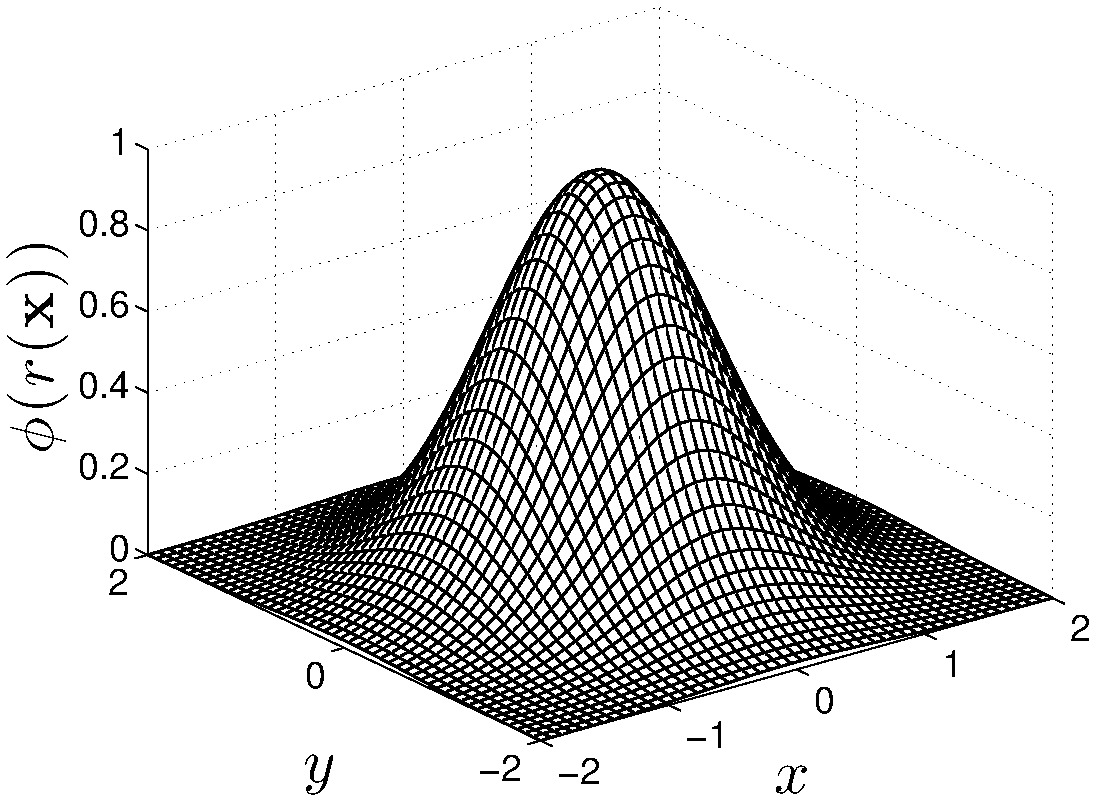
\includegraphics[width=1.0\textwidth]{../figures/paper1/figures/ga_rbf2d-eps-converted-to.pdf} 
		\caption{Gaussian}
	\end{subfigure}
	\begin{subfigure}[b]{0.25\textwidth}
	\centering
		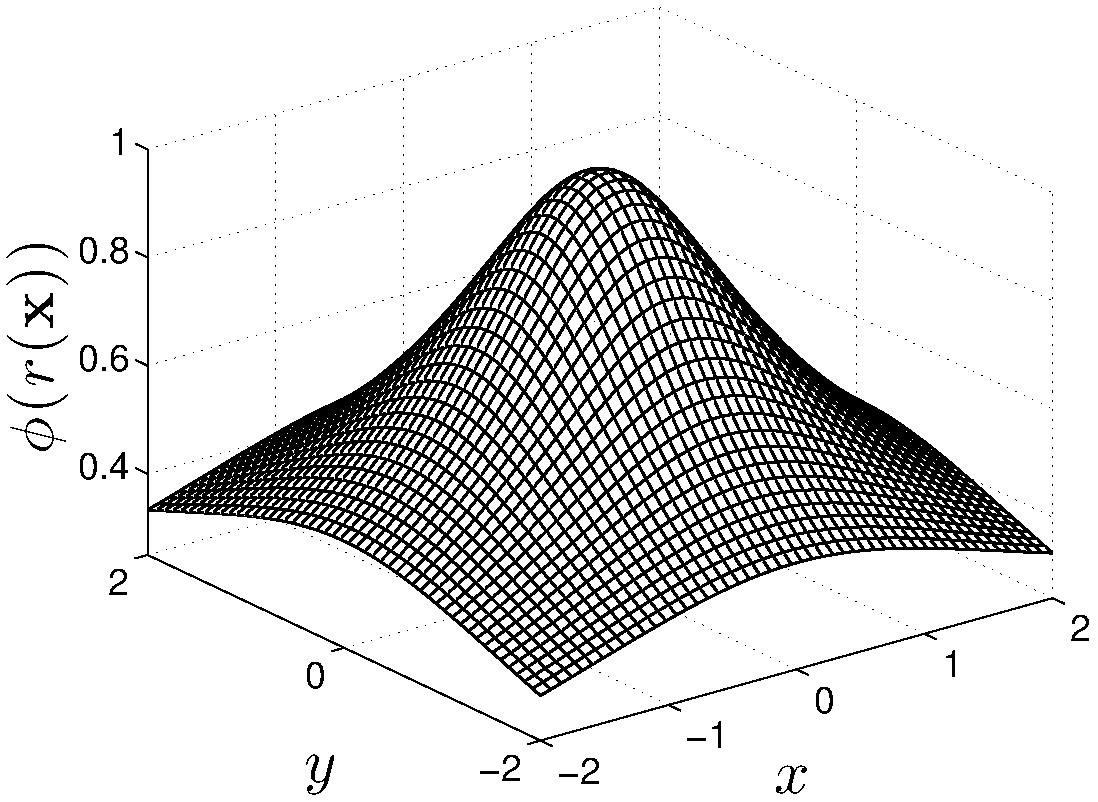
\includegraphics[width=1.0\textwidth]{../figures/paper1/figures/imq_rbf2d-eps-converted-to.pdf}
		\caption{Inverse Multiquadric}
	\end{subfigure}
	\begin{subfigure}[b]{0.25\textwidth}
	\centering
		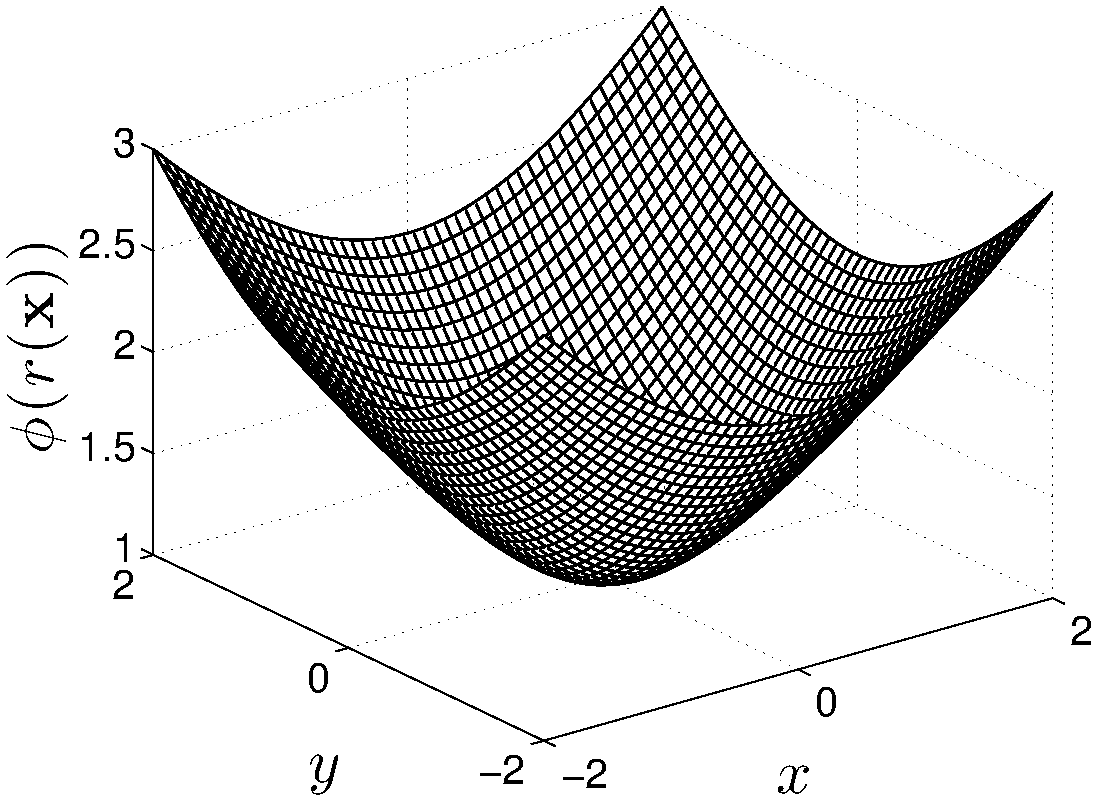
\includegraphics[width=1.0\textwidth]{../figures/paper1/figures/mq_rbf2d-eps-converted-to.pdf} 
		\caption{Multiquadric}
	\end{subfigure} 
    \caption{Commonly Used Radial Basis Functions (RBFs).}
    \label{fig:rbfs}
\end{figure}

At the core of all RBF-based PDE methods lies the fundamental problem of approximation/interpolation. Some methods (e.g., global- and compact-RBF methods) apply RBFs to approximate derivatives directly. Others (e.g., RBF-FD) leverage the basis functions to compute stencil weights, which in turn are used in generalized finite-difference approximations of derivatives. 

As ``meshless" methods, RBF methods excel at solving problems that require geometric flexibility with scattered node layouts in $d$-dimensional space. They naturally extend into higher dimensions with minimal increase in programming complexity \cite{FlyerWright07,WrightFlyerYuen10}. In addition to competitive accuracy and convergence compared with other state-of-the-art methods \cite{FlyerWright07, FlyerWright09, FlyerLehto10, WrightFlyerYuen10, FlyerFornberg11}, RBF methods boast stability for large time steps. Not all RBF methods are truly meshless. Most of them operate the same given an input set of nodes, whether or not the input includes an underlying mesh. However, some methods connect all nodes to all others (to be meshless), while methods like RBF-FD rely on stencils to connect points within small neighborhoods of one another. The generated stencils limit the scope of influence for nodes and complexity of the method, but also simulate a mesh. 

%Most literature surrounding RBF solutions for PDEs apply the concept of collocation (see Chapter~\ref{chap:background}). Recent trends in the community appear to have shifted, and RBF-FD seems to be top of the list. 


%RBF-FD is a hybrid of RBF scattered data interpolation and classical Finite Difference (FD). It shares many of the benefits from other RBF methods, like functionality on scattered node layouts in any dimension and high-order accurate solutions. Likewise, benefits akin to classical FD such as compact stencils for derivative approximation, and low computational complexity.

%Classical FD derivatives are expressed at a single node (center) as a weighted combination/difference of solution values from a small neighborhood (i.e., a stencil) around the center. Common approximations such as upwind differencing, center differencing, and other higher order approximations are of this form. 
%In similar fashion, RBF-FD combines solutions values based on stencils, but it does so in a more generalized sense than standard FD. For example, classical FD is typically restricted to regular meshes and often symmetric stencils in practice with the same set of weights for each stencil. Weights can be derived from polynomial expansion and obtained in 1D by solving a Vandermonde interpolation matrix \cite{FornbergLehto11}. Higher dimension FD stencils are composed from combinations of 1D formulas applied to each dimension. This implies restrictions on the shape/layout of stencils. In contrast to this, RBF-FD is designed for stencils with irregular node placement and can easily provide a unique set of weights for each stencil with no restrictions on stencil shape. 

%TODO:  \cite{Wright2004, Wright2003, WrightFornberg06, Chandhini2007}. 
To track the history of RBF methods, one must rewind to 1971 and R.L. Hardy's seminal research on interpolation with multi-quadric basis functions \cite{Hardy1971}. The transition from interpolation to RBF PDE methods dates back to 1990 \cite{Kansa1990a,Kansa1990b}. 
The RBF-FD method was first introduced in concept in 2000 \cite{Tolstykh2000}, but it took another few years for the method to really get a start (\cite{Shu2003}, \cite{Tolstykh2003a}, \cite{Wright2003} and \cite{Cecil2004}). Now a little over a decade old, the method is finally showing signs that it has the critical-mass following necessary for use in large-scale scientific models. At the onset of this work, most of the literature considered RBF-FD for problem sizes up to a few thousand nodes; at most into tens of thousands of nodes. Similar to most RBF methods, RBF-FD is predominantly implemented within small-scale, serial computing environments. The RBF community at-large continues to depend on MATLAB for investigation and extension development.


The goal of this dissertation is to scale RBF-FD solutions on high resolution meshes across high performance clusters, and to lead the way for its adoption within HPC and supercomputing circles. As part of this push to HPC, leveraging \emph{Graphics Processing Units (GPUs)} for computation is considered critical. GPUs, introduced in Chapter~\ref{chap:gpu_rbffd}, are many-core accelerators capable of general purpose, embarrassingly parallel computations. Driven first by the gaming industry's insatiable desire for more realistic graphics, and now also by the scientific community's demand for massive parallelism, GPU performance in the recent years has 
tremendously grown compared to CPUs. Accelerators represent the latest trend in HPC, where compute nodes are commonly supplemented by one or more accessory boards for offloading compute intensive tasks. Our effort leads the way for RBF-FD applicationss in an age when compute nodes with attached accelerator boards are considered key to breaching the exa-scale computing barrier \cite{GPUandExascale2011}. 

%We find it pertinent to clarify that this dissertation does not involve the design or study of full geophysical models. Those tasks are reserved for a computational geophysicists. We limit our focus instead to efficient parallel implementation of the numerical methods  computational geophysicist would . To verify code correctness, we test on simplified geophysical equations for the sphere. The lack of boundaries is also intentional \authnote{finish: clarify geophysics aspect}.


Parallelization of RBF-FD is achieved at two levels. On the first level, the
physical domain of the problem is partitioned
into overlapping subdomains, each handled by different MPI processes. All processes
operate independently to compute/load RBF-FD stencil weights, run diagnostic
tests and perform other initialization tasks. A process only computes weights
corresponding to stencils centered in the interior of its partition. After
initialization, processes work together to concurrently solve the PDE. Communication
barriers ensure that processes execute in lockstep and maintain consistent
solution values across the domain.  

The second level of
parallelization offloads tasks to the GPU at each iteration of the PDE solver. The bulk of computation in RBF-FD relies on a \emph{Sparse Matrix-Vector multiply (SpMV)} to evaluate derivatives. When mapped to the GPU, the SpMV operation is broken into two parts in order to overlap communication and computation, and amortize the cost of data transfer across multiple levels of hardware (see Chapter~\ref{chap:multigpu_rbffd}). 
% Although the stencil weight calculation is also data-parallel, we assume that in this context that the weights are precomputed and loaded once from disk during the initialization phase. 

%Additional key challenges lie in the choice of grid, the choice of stencil, and stability of scalable solutions. 
%To demonstrate Chapter~\ref{chap:applied_rbffd} verifies 


%
%Even today, RBFs are still up-and-coming in the scientific world with many avenues of research left to consider. Global formulations are understood to have spectral convergence properties, high accuracy and other benefits like adaptivity and ease of implementation over meshed methods \cite{Fasshauer:2007}. However, little is known about the behavior of local and RBF-FD methods. Open questions include (but are in no way limited to): a) ideal node placement to eliminate singularities; b) data-structures for stencil storage and evaluation; c) problem sizes larger than a few thousand nodes; and d) parallel implementations across new heterogeneous multi- and many-core architectures. In response to this, our group, in collaboration with researchers assembled from a national lab and four universities (see Chapter~\ref{chap:funding}), has been granted funds by the National Science Foundation to collaboratively:
%
%\begin{quote}
%\emph{``Bring RBFs to the forefront of multi-scale geophysical modeling by developing fast, efficient, and parallelizable RBF algorithms in arbitrary geometries, with performance enhanced by hardware accelerators, such as graphic processing units (GPUs)."} \cite{RBF_proposal:2009}
%\end{quote}
%
%



The layout of this document is as follows. This chapter continues with a survey of work related to parallelizing RBF-FD, targeting the GPU, and spanning a multi-GPU cluster. Chapter~\ref{chap:background} provides a historical survey of RBF methods as a backdrop to present RBF-FD in Chapter~\ref{chap:rbffd_method}. Chapter~\ref{chap:stencils} introduces a new algorithm for generating RBF-FD stencils as a faster alternative to the RBF community favorite, $k$-D Tree. In Chapter~\ref{chap:distributed_rbffd}, the first scalable implementation of RBF-FD to span one thousand processors is described in detail. Chapter~\ref{chap:gpu_rbffd} continues with the challenge of offloading computation to GPUs, and Chapter~\ref{chap:multigpu_rbffd} expands the discussion to RBF-FD on a multi-GPU cluster. In Chapter~\ref{chap:applications} the parallel RBF-FD implementation is applied and verified on the solutions of both explicit and implicit geophysical PDEs. Finally, Chapter~\ref{chap:conclusions} concludes with a summary of novel contributions, results and a discussion on future directions.

\section{Related Works: Parallel/Distributed PDE Methods} 

With the large following that RBF methods have gained since their inception in the 1970s, it is impossible to exhaustively list all 
applications, advances and related methods. Rather, this section concentrates specifically on RBFs applied to PDEs, and branches out to additional topics where necessary. %A detailed look at RBF PDE methods can be found in Chapter~\ref{chap:background}.

Table~\ref{tbl:parallel_rbf_refs} provides a number of related works classified according to the type of parallelism they exhibit. The table presents investigations from both inside and outside the RBF community partitioned into one of three types: multi-CPU, single GPU, and multi-GPU. Initial classifications are refined by parallel language/standard employed. The multi-CPU class includes any investigations that are parallelized by OpenMP, MPI, or the combination of the two, but do not include details of GPU computing. If GPUs (one or more) are used, then we categorize based on the GPU language: CUDA, OpenCL, or ``Other". The ``Other" category lumps together all languages pre-dating CUDA, including shader-based languages (e.g., GLSL, HLSL, Cg), and early streaming languages (e.g., Brook+, Sh/RapidMind). Multi-GPU implementations match each GPU with a CPU which managed communication. Communication can be overlapped, implying that the GPU continues computing on a local problem while the CPU waits on data, or non-overlapped if both the GPU and CPU wait. 

Parallel implementations of RBF methods rely on \emph{domain decomposition}. Depending on the implementation, domain decomposition not only accelerates solution procedures, but can decrease the ill-conditioning that plague all global RBF methods (\cite{Divo2007}). The ill-conditioning is reduced if each domain is treated as a separate RBF domain, and the boundary update is treated separately. Domain decomposition methods for RBFs were introduced by Beatson et al. \cite{Beatson2000}. Their work provided a solution to solve problem sizes into the millions of nodes.

This work leverages a domain decomposition; although, not for the purpose of conditioning. Instead, subdomains are distributed across multiple compute nodes and solved simultaneously. MPI communicates data dependencies across subdomain boundaries. Our implementation of RBF-FD is demonstrated to scale across more than a thousand CPU cores of an HPC cluster. In addition to high scalability for distributed computing, our novel implementation offloads computation to the GPU with an algorithm that overlaps communication and computation. This combination of multi-CPU and multi-GPU parallelism is unmatched in related work within the RBF-FD community. In fact, the multi-GPU aspect sets this work apart from the entire class of RBF methods. 

\begin{table}
    \centering
    \caption{Classification of references by numerical method and parallelization strategy.}
    \label{tbl:parallel_rbf_refs}
    \begin{tabular}{L{0.11\textwidth}||C{0.1\textwidth}|C{0.08\textwidth}||C{0.08\textwidth}|C{0.09\textwidth}|C{0.08\textwidth}||C{0.1\textwidth}|C{0.125\textwidth}||}
         % Use a star or cross to denote OpenMP + MPI. 
                                    & \multicolumn{2}{C{0.2\textwidth}||}{Multi-CPU ($^\star$:MPI+OpenMP)} & \multicolumn{3}{C{0.3\textwidth}||}{Single GPU} & \multicolumn{2}{C{0.23\textwidth}||}{Multi-GPU ($^\dag$:Non-overlapped, $^\ddag$:Overlapped)} \\ \cline{2-8}
                                    & OpenMP & MPI & CUDA     & OpenCL     & Other     & CUDA     & OpenCL   \\ \hline
             RBF-FD                 &            &         &          &            &            &          & \cite{BolligFlyerErlebacher2012}$^{\dag}$ \mbox{[This Work]$^{\ddag}$}  \\ \hline
             RBF PDE Methods  &  \cite{Kosec2008}   & \cite{Divo2005, Divo2007, Ingber2003,Ingber2004,Yokota2010} & \cite{Schmidt2009a,Schmidt2009b,Gumerov2007a, Gumerov2007b} &    &   &   &  \\ \hline
             Non-PDE RBF Methods    &         &    \cite{Strey2003}$^{\star}$      &  \cite{Cuomo2013,Cuntz2007}  &   &  \cite{Corrigan2005,Weiler2005,Carr2003,Brandstetter2008}  &   &      \\ \hline \hline
             Non-RBF PDE Methods    &     &   \cite{Schubert2011}$^{\star}$    &  \cite{Corrigan2009}  &      &      &   \cite{Goeddeke2007,Goeddeke2008a,Goeddeke2009a, Goeddeke2008b, Thibault2009, Phillips2009,Komatitsch2009}$^{\dag}$ \cite{Minden2010, YokotaGPU2010, Phillips2010,Komatitsch2010b,Komatitsch2010a}$^\ddag$ &  \\ \hline
    \end{tabular}
\end{table}

\subsection{RBF Methods on Multi-Core and Multi-CPU}

Kosec and \v{S}arler \cite{Kosec2008} have the only known (to our knowledge) OpenMP implementation for RBF PDE methods. The authors parallelize coupled heat transfer 
and fluid flow problems on a single workstation. 
The application involves the local RBF collocation method, explicit time-stepping and Neumann boundary conditions. A speedup 
factor of 1.85x over serial execution was achieved by executing on two CPU cores; no further 
results from scaling tests were provided. 

The performance and scaling of a parallel RBF neural network is tested on a SunFire 6800 SMP by Strey \cite{Strey2003}. Scaling benchmarks for OpenMP, MPI, and MPI+OpenMP versions of his code demonstrate the performance up to 12 of the 24 CPUs within the system.

Global RBF collocation method is parallelized in \cite{Ingber2003,Ingber2004} with a Schwarz Neumann-Neumann domain decomposition method to solve 3-D diffusion equations. In both cases the authors utilize MPI for communication and provide only coarse grained scaling data at 8, 27 and 64 nodes. 
 
 
Divo and Kassab \cite{Divo2005} develop a domain decomposition method with artificial 
subdomain boundaries and parallelize global RBF collocation across a small cluster of 10 compute nodes. Subdomains are processed independently, with derivative values 
at artificial boundary points averaged to maintain global consistency of physical values. The authors focus predominantly on verification of the decomposition method for heat transfer problems, and neglect thorough benchmarking and scalability testing for the MPI implementation. In \cite{Divo2007}, Divo and Kassab apply their domain decomposition to parallelize a local RBF collocation method. The method
was run on 36 node cluster, but once again benchmarks and scalability tests are not provided. 


Perhaps the most competitive parallel implementation of an RBF method is the PetRBF branch of PETSc \cite{Yokota2010}. The authors of PetRBF have implemented a highly scalable, efficient RBF interpolation method based on compact RBFs (i.e., they operate on sparse matrices). The authors demonstrate efficient weak scaling of PetRBF across 1024 processes on a Blue Gene/L, and strong scaling up to 128 processes on the same hardware. On the Blue Gene/L, PetRBF is demonstrated to achieve an impressive 74\% parallel weak scaling efficiency on 1024 processes (operating on over 50 million points), and 84\% strong scaling efficiency for 128 processes. Strong scaling was also tested on a Cray XT4, where strong scaling tops out at 36\% for 128 processes, a respectable number---and similar to observed results for our own code on for the same number of processes (see Chapter~\ref{chap:distributed_rbffd}).  


Stevens et al. \cite{Stevens2009a} mention a parallel implementation under development, but no document is available at this time. 



\subsection{RBF Methods on GPUs}


While a number of related works consider RBFs on GPUs, most of the investigations relate to visualization (e.g., \cite{Cuntz2007, Weiler2005}),  surface reconstruction (e.g., \cite{Corrigan2005,Carr2003}), and neural networks (e.g., \cite{Brandstetter2008}). Of these, only \cite{Cuntz2007} uses a modern GPGPU langauge (CUDA), the rest rely on shader languages (i.e., GLSL, HLSL, etc) denoted as ``Other" in Table~\ref{tbl:parallel_rbf_refs}.

The only known applications of GPUs to solve PDEs with RBFs are found in \cite{Gumerov2007a, Gumerov2007b} and \cite{Schmidt2009a, Schmidt2009b}. 

In the case of \cite{Schmidt2009a, Schmidt2009b}, Schmidt et al. compare implementations of a global RBF collocation scheme to a staggered leapfrog FD scheme. The authors solve the 2D (heightfield) shallow water equations for Tsunami simulation with both methods. Time-stepping is controlled by a $4^{th}$ order Runge-Kutta scheme; the same scheme is adopted here. Results for a problem size of $32\times32$ RBF centers show similar error to a $185\times 185$ staggered leapfrog discretization \cite{Schmidt2009b}. 
Their codes were written in MATLAB and leveraged the AccelerEyes Jacket \cite{JacketGuide2009} add-on to provide wrappers and data structures for internal calls to the NVidia CUDA API. The model was based on a single large dense matrix solve, and with the help of Jacket the authors were able to achieve approximately 7x speedup (no GFLOP/sec provided) over the standard MATLAB solution on the then current generation of the MacBook Pro laptop. The authors compared the laptop CPU (processor details not specified) to the built-in NVidia GeForce 8600M GT GPU. Schmidt et al.'s implementation was the first contribution to the RBF community to leverage accelerators. The results were promising, but no further contribution was made on the topic. 

In \cite{Gumerov2007a, Gumerov2007b}, Gumerov et al. designed a library of FORTRAN wrappers around CUDA that interface with existing code. The wrappers allow existing code bases to leverage GPUs with minimal modification. Wrapping the cuFFT (an FFTW implementation for the GPU \cite{CudaGuide2011}) and cuBLAS libraries the authors present accelerated implementations of both a pseudo-spectral plasma turbulence problem (nonlinear PDE), and a Fast Multipole Method that depends internally on an iterative solution to RBF interpolation. Their Fast Multipole Method is only distantly related to RBF PDE methods discussed in Chapter~\ref{chap:background}. On top of this, the implementation again depends on dense matrix algebra.


While our method and \cite{Schmidt2009a,Schmidt2009b,Gumerov2007a, Gumerov2007b} are all based on RBFs, the problems are only distantly related on the GPU. Our work relies on sparse matrix operations, while the others operate on dense matrices. Dense matrix operations have a high computational complexity and are compute-bound problems that can fully utilize the hardware. They are considered ideal (or near to) by linear algebra libraries like BLAS \cite{BLAS} and LAPACK \cite{Lapack1999}, and were demonstrated to fit well on GPUs in the early days of computer graphics, long before NVidia provided the efficient cuBLAS library \cite{CudaToolkitDoc}---a BLAS substitute on the GPU---in the initial public release of CUDA in 2006. In stark contrast to this, sparse problems have much lower computational complexity and are memory bandwidth-bound. Getting good performance on sparse problems requires an entirely different set of rules. 

Earlier this year (2013), Cuomo et al. \cite{Cuomo2013} implemented RBF-interpolation on the GPU for surface reconstruction. Their work is based on an extension of PetRBF \cite{Yokota2010}, and new built-in back-ends that allow GPU access within PETSc (\cite{Minden2010}). PETSc now internally wraps both the CUSP \cite{Cusp2012} (CUDA) and ViennaCL \cite{Rupp2010,Rupp2010a} (OpenCL) projects for sparse matrix algebra on the GPU. With the help of the CUSP backend, Cuomo et al. solve and apply sparse interpolation systems on the GPU for up to three million nodes on an NVidia Fermi C1060 GPU (4GB). They compare results to a single core CPU implementation on an Intel i7-940 CPU and demonstrate that the GPU accelerate their solutions between 6x and 25x. Unfortunately, the authors do not show any evidence of scaling the interpolation to multiple GPUs. Therefore, while evidence exists that PetRBF now has full GPU support, its scalability remains an open question. 


Aside from our own investigations, no known efforts apply the GPU to the RBF-FD method. 


\subsection{Non-RBF Methods} 

\authnote{Need to expand on this section} 

A number of multi-GPU implementations unrelated to RBF methods can provide context for the relevancy of our research.

%First, a single-GPU finite-volume implementation is introduced by Corrigan et al. in \cite{Corrigan2009} to solve 3D incompressible fluid problems on an unstructured grid. Within their GPU kernels, each element of the unstructured mesh is operated on by a single thread---this design is equivalent to our ``one thread per stencil" test case in Chapter~\ref{chap:gpu_rbffd}. The author's effort to operate on unstructured grids posed a challenge, in that the unstructured elements with random ordering caused considerable slow-down on the GPU due to non-coalesced memory loads. In response to this, Corrigan et al. reorder their meshes with a fixed-grid method similar to our approach in Chapter~\ref{chap:stencils}.

One of the earliest multi-GPU implementations, presented in a series of articles \cite{Goeddeke2007, Goeddeke2008a, Goeddeke2008b, Goeddeke2009a} by G\"{o}ddeke et al. introduced
a GPU enhanced version of the pre-existing parallel (MPI) multigrid finite element package, FEAST. In \cite{Goeddeke2007} the authors integrated 
GPUs in a minimally invasive fashion (e.g., farming out local multigrid tasks to the GPU) and considered the weak scalability (i.e., 
increasing the number of co-processors while keeping the problem size fixed on each processor) on up to 160 compute nodes with a 
single GPU each.  Since the accelerated routines were implemented below the original FEAST API, it was demonstrated in 
\cite{Goeddeke2008a} that existing applications built on top of the original FEAST could benefit without code modifications when 
the 
new package, FEASTGPU, was substituted. \cite{Goeddeke2008b} compared performance of single-,  double- and 
mixed-precision calculation within FEASTGPU. \cite{Goeddeke2009a} applied FEASTGPU to nonlinear Navier-Stokes 
problems and 
found the minimally invasive approach had limited impact on performance in the new setting where computational work was no longer  
concentrated in GPU-accelerated tasks. 

At roughly the same time other efforts around the world started targeting multi-GPU clusters, opting first for non-overlapped communication only to realize the necessity for overlap in order to increase parallel efficiency. 
For example, Phillips et al. \cite{Phillips2009} draw this conclusion based on scaling of their finite-volume method for compressible flow equations on an irregular structured grid on eight quad-core workstations with a total of 32 GPUs. 
Thibault et al. \cite{Thibault2009} also note the need for overlap when modeling 3D incompressible fluids with finite differencing on structured grids and multiple GPUs. Their solutions to the lid-driven cavity problem are based on a Jacobi iteration. 


Komatitsch et al. \cite{Komatitsch2009,Komatitsch2010b,Komatitsch2010a} demonstrated overlapping communication and computation on GPUs within the SPECFEM3D package. With the help of non-blocking MPI communication and a sufficiently large problem, roughly 90\% of communication time can be hidden. 

Phillips and Fatica overlap communication and computation in \cite{Phillips2010} while solving the Himeno benchmark, a test specifically designed to compare performance of processors based on a memory bound application (in this case the 3-D Poisson problem in generalized coordinates).  


Most recently, the latest version of PETSc now includes GPU support \cite{Minden2010,YokotaGPU2010}. PETSc is a widely-used library for distributed sparse and dense matrix algebra, with proven scalability on many supercomputing clusters. A large number of libraries like \authnote{examples} depend on PETSc internally for computation. 


%Meshed methods have received a large amount of attention from the GPU community. For example, Bolz et al. \cite{Bolz2003} implemented conjugate gradient and multigrid kernels for 2D FD incompressible fluid simulation using FD on a single GPU.  More recently, a single GPU, multigrid finite-difference based solver was applied to 3D compressible fluid flow (Euler equations) by Elsen et al. \cite{Elsen2008}.


\section{Major Contributions}

Within this document readers should expect to find the following major contributions: 
\begin{enumerate} 
\item The first ever application of a fixed-grid neighbor query algorithm (popularized by distantly related particle methods) to generate stencils for RBF-FD. 
\begin{itemize} 
\item Performance comparison with the RBF community favorite, $k$-D Tree, shows that the lower complexity fixed-grid method is able to achieve up to 2.5x speedup over the former method on randomly distributed nodes. 
\item The fixed-grid method is also shown to accelerate RBF-FD time-step performance by up to 5x due spatial locality of node information in memory and improved cache effects.
\end{itemize} 
\item Integer dilation and bit interleaving are introduced to the RBF community at large to construct a number of space-filling curve variants in 2-D and 3-D. The curves reorder cells of the fixed-grid algorithm on the prospect of additional cache hits for derivative calculations. 
\begin{itemize} 
\item A comparison of the variants to the result of the well-known Reverse Cuthill-McKee (RCM) algorithm concludes that RCM remains the better option for reordering and matrix bandwidth minimization.
\end{itemize} 
\item The design and tuning of the only known implementation of the RBF-FD method to scale across multiple compute nodes of a supercomputing cluster.
\begin{itemize} 
\item Our home-grown implementation divides computation with a Restricted Additive Schwarz (RAS) domain decomposition in a first-of-its-kind application to RBF-FD. % (note: other RBF methods have already encountered RAS decomposition \cite{Yokota2010}). 
\item As part of the tuning process described herein, balanced workloads are achieved through the use of the METIS graph partitioning algorithm \cite{Karypis1999}.  
\item A number of steps are taken to improve communication collectives in the CPU-only implementation. The resulting algorithm splits derivative calculation into two steps and overlaps communication with computation. We observe that up to 80\% of the cost in communication can be hidden in some cases. 
\item Scaling benchmarks up to 1024 processes (divided into 8 processes per node) and a grid resolution of $N=160^3$ vertices (i.e., 4.1 million) prove that the implementation scales well in both a strong and weak sense. 
\end{itemize} 
\item The design and tuning of the only known single- and multi-GPU implementation of RBF-FD. Also, ours is the only known investigation in the broader RBF community to target multiple GPUs. 
\begin{itemize} 
\item Our first paper (\cite{BolligFlyerErlebacher2012}) introduced a set of custom OpenCL kernels for RBF-FD time-stepping of hyperbolic PDEs with an explicit RK4 scheme (up to 10 GPUs). 
\item Here, the performance per GPU is tuned by choosing an alternative sparse matrix representation. The investigation reveals that the Ellpack (ELL) structure provided by the ViennaCL library \cite{Rupp2010} is a great fit for RBF-FD differentiation matrices, with over 4x faster performance than the original compressed-row storage (CSR). %On one GPU (NVidia M2070) our implementation performs at approximately 8 GFLOP/sec. 
\item The multi-GPU implementation is extended to a novel overlapping algorithm that naturally derives from our distributed CPU optimizations. Non-blocking MPI collectives plus two asynchronous OpenCL queues amortize the cost of data transfer between CPU and GPU, MPI communication, and in some cases a substantial amount of computation. Iterations of the resulting implementation achieve an average of 3x improvement in strong scaling compared to a non-overlapping equivalent. 
\end{itemize} 
\end{enumerate}
Of lesser significance we also: 
\begin{enumerate}
\item Verify our explicit solvers against two well studied hyperbolic PDEs (Vortex Roll-up \cite{NairTransport05, NairJablonowski08} and Cosine Bell Advection \cite{JakobChien1995}).
\begin{itemize} 
\item Convergence studies confirm that hyperviscosity (\cite{Fornberg2011b}) stabilizes solutions.
\item Tuned parameters are provided for selecting the RBF support parameter and scaling hyperviscosity as a function of the problem size
\end{itemize}
\item Implement a distributed multi-GPU preconditioned GMRES within ViennaCL for implicit RBF-FD solutions.
\begin{itemize} 
\item A divergence-free field is constructed as the manufactured solution for a simplified version of Stokes flow constrained to the unit sphere. 
\item Contributed a CPU-only preconditioner (Incomplete LU with Zero Fill-in) to ViennaCL to test impact on GMRES convergence rates 
\end{itemize}
\item Provide preliminary benchmarks evaluating the performance of RBF-FD on the Intel Phi Architecture. 
%\begin{itemize} 
%\item We leverage the cross-platform functionality of OpenCL to operate in Offload Mode on the Phi with the latest Beta OpenCL driver from Intel. 
%\end{itemize}
\end{enumerate}



\ifstandalone
%Bei direkter Übersetzung sollte gleich noch das Literaturverzeichnis rein.
\bibliographystyle{plain}
\bibliography{merged_references}
\end{document}
\else
\expandafter\endinput
\fi
